% mnras_template.tex
%
% LaTeX template for creating an MNRAS paper
%
% v3.0 released 14 May 2015
% (version numbers match those of mnras.cls)
%
% Copyright (C) Royal Astronomical Society 2015
% Authors:
% Keith T. Smith (Royal Astronomical Society)

% Change log
%
% v3.0 May 2015
%    Renamed to match the new package name
%    Version number matches mnras.cls
%    A few minor tweaks to wording
% v1.0 September 2013
%    Beta testing only - never publicly released
%    First version: a simple (ish) template for creating an MNRAS paper

%%%%%%%%%%%%%%%%%%%%%%%%%%%%%%%%%%%%%%%%%%%%%%%%%%
% Basic setup. Most papers should leave these options alone.
\documentclass[fleqn,usenatbib]{mnras}
%\pdfminorversion=5

% MNRAS is set in Times font. If you don't have this installed (most LaTeX
% installations will be fine) or prefer the old Computer Modern fonts, comment
% out the following line
%\usepackage{newtxtext,newtxmath}
% Depending on your LaTeX fonts installation, you might get better results with one of these:
%\usepackage{mathptmx}
%\usepackage{txfonts}

% Use vector fonts, so it zooms properly in on-screen viewing software
% Don't change these lines unless you know what you are doing
\usepackage[T1]{fontenc}
\usepackage{ae,aecompl}
\usepackage{hyperref}

%%%%% AUTHORS - PLACE YOUR OWN PACKAGES HERE %%%%%

% Only include extra packages if you really need them. Common packages are:
\usepackage{graphicx}	% Including figure files
\usepackage{amsmath}	% Advanced maths commands
\usepackage{amssymb}	% Extra maths symbols
\usepackage{multirow}
\usepackage[usenames,dvipsnames,svgnames,table]{xcolor}
\usepackage{verbatim}

%\hypersetup{draft}

%%%%%%%%%%%%%%%%%%%%%%%%%%%%%%%%%%%%%%%%%%%%%%%%%%

%%%%% AUTHORS - PLACE YOUR OWN COMMANDS HERE %%%%%

% Please keep new commands to a minimum, and use \newcommand not \def to avoid
% overwriting existing commands. Example:
%\newcommand{\pcm}{\,cm$^{-2}$}	% per cm-squared

\newcommand{\homsun}{\,h^{-1} {\rm M_\odot}}
\newcommand{\hmsun}{\,h^{-2} {\rm M_\odot}}
\newcommand{\msun}{{\rm M_\odot}}
\newcommand{\hkpc}{\, h^{-1}{\rm{kpc}} }
\newcommand{\hMpc}{\, h^{-1}{\rm{Mpc}} }
\newcommand{\magn}{\, {\rm mag} }

\newcommand{\hsmsun}{\,h_{70}^{-2} {\rm M_\odot}}
\newcommand{\hskpc}{\, h_{70}^{-1}{\rm{kpc}} }
\newcommand{\hsMpc}{\, h_{70}^{-1}{\rm{Mpc}} }
\newcommand{\hsGpc}{\, h_{70}^{-1}{\rm{Gpc}} }

\newcommand{\lan}{\langle}
\newcommand{\ran}{\rangle}

\newcommand{\lcdm}{{\rm \Lambda CDM}}
\newcommand{\am}{\, {\rm arcmin}}
\newcommand{\as}{\, {\rm arcsec}}
\newcommand*{\mean}[1]{\overline{#1}}
\newcommand*{\E}[1]{\times 10^{#1}}
\newcommand{\un}[1]{_{\rm #1}}

\newcommand*{\swap}[2]{#2#1}

%%%%%%%%%%%%%%%%%%%%%%%%%%%%%%%%%%%%%%%%%%%%%%%%%%

%%%%%%%%%%%%%%%%%%% TITLE PAGE %%%%%%%%%%%%%%%%%%%

% Title of the paper, and the short title which is used in the headers.
% Keep the title short and informative.
\title[Extending the RAR with KiDS weak lensing]{Extending the Radial Acceleration Relation using Weak Gravitational Lensing with the Kilo-Degree Survey}
% The list of authors, and the short list which is used in the headers.
% If you need two or more lines of authors, add an extra line using \newauthor
\author[M. M. Brouwer et al.]{Margot M. Brouwer$^{1,2}$\thanks{E-mail:brouwer@astro.rug.nl},
	 %Group 1:
	 %Group 2:
	 %Group 3:
	\\
	\\
	% List of institutions
	$^{1}$Kapteyn Astronomical Institute, University of Groningen, PO Box 800, NL-9700 AV Groningen, the Netherlands.\\
	$^{2}$Institute for Theoretical Physics, University of Amsterdam, Science Park 904, 1098 XH Amsterdam, The Netherlands. \\
}

% These dates will be filled out by the publisher
\date{Accepted XXX. Received YYY; in original form ZZZ}

% Enter the current year, for the copyright statements etc.
\pubyear{2019}

% Don't change these lines
\begin{document}
\label{firstpage}
\pagerange{\pageref{firstpage}--\pageref{lastpage}}
\maketitle

% Abstract of the paper
\begin{abstract}
TBW
\end{abstract}


% Select between one and six entries from the list of approved keywords.
% Don't make up new ones.
\begin{keywords}
gravitational lensing: weak -- Surveys -- methods: statistical -- galaxies: haloes -- cosmology: dark matter, theory -- gravitation.
\\
\end{keywords}

%\newpage
\clearpage

%%%%%%%%%%%%%%%%%%%%%%%%%%%%%%%%%%%%%%%%%%%%%%%%%%

%%%%%%%%%%%%%%%%% BODY OF PAPER %%%%%%%%%%%%%%%%%%


\section{Introduction}
\label{sec:introduction}

It has been known for several decades that the outer regions of galaxies rotate faster than would be expected from Newtonian dynamics based on their luminous, or `baryonic', mass. This was first discovered by \cite{rubin1983} through measuring galactic rotation curves of optical disks, and by \cite{bosma1981} through measuring hydrogen profiles at radii beyond the disk. The excess gravity implied by these measurements has been generally attributed to an unknown and invisible substance named Dark Matter (DM), a term coined more than forty years prior by \cite{zwicky1937} when he discovered the so-called `missing mass problem' through the dynamics of galaxies in clusters.

Following more recent observations using Weak gravitational Lensing \cite[WL,][]{hoekstra2004,linden2014,mandelbaum2015}, Baryon Acoustic Oscillations \cite[BAO's,][]{eisenstein2005,blake2011} and the Cosmic Microwave background \cite[CMB,][]{spergel2003,planck2014}, Cold Dark Matter\footnote{DM particles that moved at non-relativistic speeds at the time of recombination, as favoured by measurements of the CBM \cite[]{planck2014} and the Lyman-$\alpha$ forest \cite[]{viel2013}.} (CDM) became a key ingredient of the current standard model of cosmology: the $\lcdm$ model. In this paradigm, CDM accounts for $\Omega_{\rm CDM}=0.266$ of the critical density in the Universe, while baryonic matter only accounts for $\Omega_{\rm CDM}=0.049$ \cite[]{planck2018}. The cosmological constant $\Lambda$, which is necessary to explain the accelerated expansion of the Universe and is usually associated with Dark Energy (DE), accounts for $\Omega_{\rm \Lambda}=0.685$.

Although the $\lcdm$ model successfully describes the behavior of DM on a wide range of scales, no conclusive evidence for the existence of DM particles has been found so far \cite[despite years of enormous effort; for an overview, see][]{bertone2005,bertone2018}. This still leaves some room for alternative theories of gravity, such as Modified Newtonian Dynamics  \cite[MOND,][]{milgrom1983} and the more recent theory of Emergent Gravity \cite[EG,][]{verlinde2016}. In these theories particle DM does not exist, and all gravity is due to the baryonic matter (or, in the case of EG, the interaction between baryons and the entropy associated with DE). Hence, one of the main properties of these theories is that the mass discrepancy in galaxies correlates strongly with their baryonic mass distribution.

Such a correlation has indeed been widely observed. First astronomers discovered the Tully-Fisher relation \cite[TFR,][]{tully1977} between the luminosity of a spiral galaxy and its asymptotic rotation velocity \cite[]{pierce1988,bernstein1994}. Since this corresponds to a relation between the baryonic and the total galaxy mass, this has later been named the `baryonic' TFR \cite[BTFR,][]{mcgaugh2000,mcgaugh2012}. As the radial resolution of observations increased, astronomers found a strong correlation between the observed rotation velocity $v\un{obs}(r)$ as a function of galaxy radius $r$, and the enclosed luminous mass \mbox{$M\un{b}(<r)$} \cite[]{sanders1986,sanders1996,mcgaugh2004,sanders2007,wu2015}. Since $M\un{b}(<r)$ corresponds to the \emph{expected} gravitational acceleration $g\un{b}(r)$ from baryonic matter, and the observed gravitational acceleration can be calculated through $g\un{obs}(r)=v\un{obs}^2(r)/r$, this relation has been named the Radial Acceleration Relation (RAR)\footnote{Another well-established name for this same relation is the Mass-Discrepency Acceleration Relation (MDAR), which refers to the correspondance between the observed baryonic/total mass and the inferred mass discrepency commonly attributed to DM. Throughout this work we use the term RAR for brevity.}.

Particularly, the latest results from \cite{mcgaugh2016} (hereafter M16) have measured the RAR relation with unprecedented accuracy, using the Spitzer Photometry and Accurate Rotation Curves \cite[SPARC,][]{lelli2016b} data of 153 late-type galaxies. Their results showed a tight correlation between $g\un{obs}$ and $g\un{bar}$, which they could fit using a simple double power law (Eq. 4 in M16) depending only on $g\un{bar}$ and one free parameter: the acceleration scale $g\un{\dagger}$ where Newtonian gravity appears to break down. This sparked the interest of scientists working on alternative theories of gravity, but also of those in favor of a statistical explanation of the RAR within the $\lcdm$ framework \cite[]{keller2017,desmond2017,ludlow2017}.

The latter possibility was quantified by \cite{navarro2017} (hereafter N17) who used a range of simplifying assumptions based on galaxy observations and DM simulations, in order to create an analytical galaxy+halo model. The goal of their model was to reconstruct the RAR in galaxies, in particular the value of $a\un{0}$: the acceleration scale where the relation transitions from the baryon-dominated to the DM-dominated regime (which is equivalent to $g\un{\dagger}$), and $a\un{min}$: the minimum acceleration probed by galaxy disks. Based on their results, they claimed that the RAR can be explained within the $\lcdm$ framework, at the accelerations probed by galaxy rotation curves (i.e. $g\un{obs}>a\un{min}$). However, since their model relies on the fact that luminous kinematic tracers in galaxies only probe a limited radial range, N17 predicted that extending observations to radii beyond the disk (which correspond to lower gravitational accelerations) would lead to systematic deviations from the simple relation posed by M16.

The goal of this work is to extend observations of the RAR to lower accelerations, which are not measurable using galaxy rotation curves. To this end we use gravitational lensing: the perturbation of light inside a gravitational potential as described by General Relativity (GR). In particular, we use the method of Galaxy-Galaxy Lensing (GGL): the statistical measurement of the coherent image distortion (shear) of a field of background galaxies by the gravitational potential of a sample of foreground galaxies \cite[for examples, see e.g.][]{fischer2000ggl,hoekstra2004,mandelbaum2006,uitert2016}. Using GGL we can measure the average (apparent) density distribution of galaxies up to a radius of $3\,{\rm Mpc}$, roughly a $100$ times larger than the radius of the luminous disk ($\sim 30\,{\rm kpc}$), corresponding to a value of $g\un{bar}$ that is $3$ orders of magnitude lower than those measurable with galaxy rotation curves.

First, we measure the baryonic and total density profiles of our galaxies through their luminosities and GGL profiles. These measurements will be performed using photometric data from Sloan Digital Sky Survey \cite[SDSS,]{abazajian2009} and the VISTA Kilo-Degree Infrared Galaxy survey \cite[VIKING]{edge2013}, and WL data from the Kilo-Degree Survey \cite[KiDS;][]{dejong2013}. We then translate these measurements into the baryonic and observed radial accelerations, $g\un{bar}$ and $g\un{obs}$. Finally, we compare the resulting RAR to predictions from different modified gravity theories (MOND and EG) and $\lcdm$.

The $\lcdm$ predictions will not only be provided by the N17 analytical model, but also by two mock galaxy catalogues based on two different DM simulations. One is the Marenostrum Institut de Ci{\`e}ncies de l'Espai (MICE) Galaxy and Halo Light-cone catalog \cite[]{carretero2015,hoffmann2015}, which is based on the MICE Grand Challenge lightcone simulation \cite[MICE-GC,][]{fosalba2015a,fosalba2015b,crocce2015}. The other mock galaxy catalog is based on a suite of large-volume cosmological hydrodynamical simulations, which is called the BAryons and HAloes of MAssive Systems (BAHAMAS) project \cite[]{mccarthy2017}. Our final goal is to distinguish which of the aforementioned predictions best describe the RAR at lower accelerations.

Having over ... foreground galaxies at our disposal, we are able to select specific galaxy samples designed to optimally test these predictions. Particularly, we note that most models (MOND, EG, and the N17 analytical DM model) focus on the description of individual, isolated galaxies. In order to test them, therefore, we select a sample of galaxies whose lensing profiles are not affected by their neighbors within the radius of our measurement. In contrast, the predictions from the MICE and BAHAMAS simulations can be tested for both isolated and non-isolated galaxy samples.

Furthermore, we note that all models give a specific prediction regarding the dependence of the RAR on baryonic galaxy mass. According to the MOND and EG theories, the relation between $g\un{bar}$ and $g\un{obs}$ should remain intact in the regime beyond the disk, independent of the disk mass. Within the $\lcdm$ paradigm, however, all predictions (analytical and simulated) are based on a `stellar-to-halo-mass relation' which is not constant as a function of baryonic galaxy mass. By splitting our foreground galaxies into bins of increasing stellar mass, we are able to better distinguish the predictions of these different models.

Our paper is structured as follows: In Sect. \ref{sec:data} we introduce our main datasets: both the KiDS and GAMA galaxy surveys which are used to perform the GGL measurements, and the MICE and BAHAMAS simulations \& mock galaxy catalogues to which we compare our results. Sect. \ref{sec:analysis} describes our analysis of these (mock) datasets as we select our isolated foreground galaxy sample, perform the GGL measurements, and translate the results into the RAR. Sect. \ref{sec:predictions} contains a description of the theoretical predictions to which we compare our observations: MOND, EG and the N17 analytical DM model. In Sect. \ref{sec:results} we present the resulting RAR measurements and model comparison. Sect. \ref{sec:discon} contains the discussion and conclusion.

Throughout this work we adopt the WMAP 9-year \cite[]{hinshaw2013} cosmological parameters : $\Omega_{\rm m}=0.2793$, $\sigma_8=0.821$, $\Omega_{\rm \Lambda}=0.7207$, and $H_0 = 70 \, {\rm km \, s^{-1} Mpc^{-1}}$, which were used as the basis of the BAHAMAS simulation.
The cosmological parameters used in creating the MICE-GC simulations are: $\Omega_{\rm m}=0.25$, $\sigma_8=0.8$, $\Omega_{\rm \Lambda}=0.75$, and $H_0 = 70 \, {\rm km \, s^{-1} Mpc^{-1}}$.
Throughout the paper we use the reduced Hubble constant $h_{70} \equiv \ H_0 / (70 \, {\rm km \, s^{-1} Mpc^{-1}})$.

\begin{comment}
Points:

- Using the WL method, we can measure the (apparent) mass distribution of galaxies up to a radius that is $\sim100$ times larger than the radius of the galaxy itself, corresponding to an acceleration scale that is 4 orders of magnitude lower than $a_min$.
- By using the unadulterated WL equations to measure the (apparent) density distribution around foreground galaxies, we necessarily assume that the laws of GR hold with respect to the deflection of light by a gravitational potential.
- In EG, this is explained by the fact that... In MOND ...
- In Section ... we will ...
\end{comment}


\section{Data}
\label{sec:data}

\subsection{KiDS source galaxies}
\label{sec:kids}

We use Galaxy-Galaxy Lensing (GGL) to measure the gravitational potential around a sample of foreground galaxies (lenses), by measuring the image distortion (shear) of a field of background galaxies (sources). These sources are observed using OmegaCAM \cite[]{kuijken2011}: a 268-million pixel CCD mosaic
camera mounted on the VLT Survey Telescope \cite[]{capaccioli2011}. Over the past seven years these instruments have performed KiDS, a photometric survey in the $ugri$ bands, which is especially designed to perform WL measurements \cite[]{dejong2013}.

GGL studies with KiDS have hitherto been performed in combination with the spectroscopic GAMA survey (see Sect. \ref{sec:gama} below). Already since the previous data release \cite[KiDS-DR3,][]{dejong2017} the KiDS survey completely covers the $286 \deg^2$ GAMA area. Although the final survey will span 1350 $\deg^2$ on the sky, the current state-of-the-art is the 4th Data Release \cite[KiDS-DR4,][]{kuijken2019} containing observations from 1006 square-degree survey tiles. The measurement of the source shapes and photometric redshifts are performed in similar fashion to \cite{dejong2017}. Changes and improvements to these methods are described in \cite{kuijken2019}. 

The measurements of the galaxy shapes are based on the $r$-band data, since this filter was used during the darkest time (moon distance $> 90 \deg$) and with the best atmospheric seeing conditions ($<0.8 \as$). The $r$-band observations are co-added using the {\scshape Theli} pipeline \cite[]{erben2013}, which is improved through the addition of an illumination correction. From these images the galaxy positions are detected through the {\scshape SExtractor} algorithm \cite[]{bertin1996}. After detection, the shapes of the galaxies are measured using the \emph{lens}fit pipeline \cite[]{miller2007,miller2013}, which includes a self-calibration algorithm based on \cite{fenechconti2017}.

The $u$, $g$ and $i$ bands are observed for the purpose of creating the photometric redshift and stellar mass estimates. In addition, the  VISTA Kilo-degree INfrared Galaxy survey \cite[VIKING,][]{edge2013} performed on the VISTA telescope adds the $ZYJHK_{\rm s}$ bands. All bands are reduced and co-added using the Astro-WISE pipeline \cite[]{mcfarland2013}. The galaxy colours, which form the basis of the photometric redshift measurements, are measured from these images using the Gaussian Apertrue and PSF pipeline \cite[GAaP][]{kuijken2008,kuijken2015}.

The addition of the lower frequency VISTA data allows us to extend the redshift estimates out to $0.1<z\un{B}<1.2$ (instead of $0.1<z\un{B}<0.9$ in KiDS-DR3), where $z\un{B}$ is the best-fit photometric redshift of the sources \cite[]{benitez2000,hildebrandt2012}. However, when performing our lensing measurements (see \ref{sec:lensing}) we use the total redshift probability distribution $n\un{z}$ of the full source population. This $n\un{z}$ is calculated using the direct calibration method \cite[DIR,][]{hildebrandt2017}, and circumvents the inherent bias related to photometric redshift estimates of individual sources.

\subsection{GAMA foreground galaxies}
\label{sec:gama}

Although the final RAR measurements will be performed using exclusively the KiDS-1000 data, the set of foreground galaxies observed by the spectroscopic GAMA survey \cite[]{driver2011} function both as a model and validation sample for the KiDS foreground galaxies. The survey was performed by the Anglo-Australian Telescope with the AAOmega spectrograph, and targeted more than $180 \, 000$ galaxies that were selected from SDSS. For this study we use the GAMA II data release \cite[]{liske2015} consisting of three equatorial regions (G09, G12 and G15). These regions span a total area of $\sim180 \deg^2$ on the sky, completely overlapping with KiDS.

GAMA has a redshift range of $0<z<0.5$, with a redshift completeness of $98.5\%$ down to Petrosian r-band magnitude $m\un{r} = 19.8 \magn$. We limit our GAMA foreground sample to galaxies with the recommended redshift quality: $n\un{Q}\geq3$. This smaller sample of spectroscopic redshifts are used to train the photometric machine-learning (ML) redshifts of our larger sample of KiDS foreground galaxies (see Sect. \ref{sec:gamalike_kids}). Despite being smaller, GAMA's accurate redshifts are highly advantageous when measuring the ESD profiles of galaxies (see Sect. \ref{sec:lensing}). Also, in combination with its high redshift completeness, GAMA allows for a better application of the isolation criterion. We therefore check that the results from the KiDS-only measurements are consistent with those from KiDS-GAMA at all times.

To measure RAR with KiDS-GAMA, we need individual stellar masses $M\un{*}$ for each GAMA galaxy. These are measured from their $ugrizZYJHK$ spectral energy distributions\footnote{The spectral energy distributions are constrained to the rest frame wavelenght range $3000-110000$ \AA.} measured by SDSS and the VISTA Kilo-Degree Infrared Galaxy survey \cite[VIKING,][]{edge2013}, by fitting them with \cite{bruzual2003} stellar population synthesis models. Following the procedure described by \cite{taylor2011}, we account for flux falling outside the automatically selected aperture using the `flux-scale' correction.

\subsection{KiDS foreground selection}
\label{sec:gamalike_kids}
Still need to know:
\begin{itemize}
	\item Maciek's GL-KiDS selection criteria for K1000.
	\item Angus' stellar mass method for K1000.
\end{itemize}

\subsection{MICE mock galaxies}
\label{sec:mice_mocks}

In order to compare our observations to predictions from $\lcdm$, we adopt two different DM simulations. One of these is the MICE-GC $N$-body simulation, which contains $\sim 7$$\E{10}$ DM particles in a $(3072 \hsMpc)^3$ comoving volume \cite[]{fosalba2015b}. From this simulation the MICE collaboration constructed a $\sim5000\deg^2$ lightcone with a maximum redshift of $z=1.4$. The DM halos in this lightcone are identified using a Friend-of-Friend (FOF) algorithm on the particles. Halos are considered `resolved' down to 20 particles, corresponding to a halos with a mass of $6\E{11} \hsmsun$. The DM halos were populated with galaxies using a hybrid Halo Occupation Distribution (HOD) and Halo Abundance Matching (HAM) prescription \cite[]{carretero2015,crocce2015}.

Every galaxy has sky coordinates, redshifts, comoving distances, apparent magnitudes and absolute magnitudes assigned to them. We use the SDSS apparent $r$-band magnitudes $m\un{r}$, as these most closely match those from KiDS \cite[see][]{brouwer2018}. We can therefore limit the MICE galaxies to the same apparent magnitude as the GL-KiDS sample: $m\un{r}<20.2 \, {\rm mag}$, in order to create a GL-MICE foreground galaxy sample. We also use the same redshift limit: $z<0.5$. The absolute magnitudes of the mock galaxies go down to $M\un{r}<-18.9$ (*should we apply a cut here?*). In the MICECATv2.0 catalogue\footnote{The MICECATv2.0 catalogue is available through CosmoHub (\url{https://cosmohub.pic.es}).} which we use in this work, each galaxy is also assigned a stellar mass $M\un{*}$ needed in order to compute the RAR (see Sect. \ref{sec:conversion}). These stellar masses are determined from the galaxy luminosities $L$ using \cite{bell2001} $M/L$ ratios.

In addition, each galaxy has a pair of lensing shear values associated with it ($\gamma_1$ and $\gamma_2$, with respect to the Cartesian coordinate system). These shear values were calculated from healpix weak lensing maps that were constructed using the `onion shell method' \cite[]{fosalba2008, fosalba2015a}. The lensing map of MICECATv2.0 has an improved resolution of $0.43 {\rm arcmin}$, which is almost twice smaller than that of MICECATv1.0. The MICE shears allow us approximate the lensing analysis we perform on our KiDS data (as described in Section \ref{sec:lensing}) using the MICE simulation. To create a sample of MICE background galaxies for the lensing analysis, we apply limits on the MICE mock galaxies' redshifts and apparent magnitudes which are analogous to those applied to the KiDS source sample: $0.1 < z < 0.9$, $m\un{r}>20$ (see \citealt{hildebrandt2017} and Sect. \ref{sec:kids}; note that uncertainties in the KiDS $z\un{B}$ are not accounted for in this selection). We also apply an absolute
magnitude cut of $M\un{r}>−19.3 \, {\rm mag}$, in order to resemble the KiDS source redshift
distribution more closely.

The MICE-GC mock catalogue also features very accurate clustering. At lower redshifts ($z<0.25$) the clustering of the mock galaxies as a function of luminosity is constructed to reproduce the SDSS clustering observations \cite{zehavi2011}, while at higher redshifts (0.45<z<1.1) it was validated against Cosmic Evolution Survey \cite[COSMOS,][]{ilbert2009}. This makes MICE especially suitable to reproduce the RAR at larger scales where neighboring galaxies start to affect the lensing signal, and to test criteria on galaxy the isolation (see Section \ref{sec:isolation}).

Because the MICE mock catalogue consists of one large realization, it is not possible to estimate the covariance matrix on the measured lensing signal. However, we can split this realization into multiple smaller areas in order to estimate the `sample variance': the difference between astrophysical measurements from different parts of the sky.

%In order to obtain a rough estimate of the mentioned uncertainties, we split the MICE-GC public lightcone area into 16 patches of 20×20 = 400 deg2 (approximately the same size as the used KiDS area). Comparing the results obtained from the full lightcone area with those of the 16 sub-samples provides an estimate of the sample variance within the MICE mocks.

% The MICE-GC simulation resolves DM halos down to a mass of 6×10^11 h_70^-2 Msun (corresponding to 20 particles), which host galaxies with an absolute magnitude < −18.9. Since this absolute magnitude includes a cosmology correction such that: M r,MICE = M r − 5 log 10 (h), where h = 0.7 is their reduced Hubble constant, we apply an M r < −18.9 − 0.77 = −19.67 mag cut to the GAMA and GL-KiDS samples in order to resemble the mock galaxy population.

% The HOD model MICE starts from the galaxy luminosity function and then converts it to stellar masses: for ‘-c01’ this conversion has been updated to obtain a better fit to the provided SMF at z= 0. For ‘-c02’ this has been implemented even more self-consistently for all redshiftswhile also changing the calibration of the star formation rate.

\subsection{Bahamas mock galaxies}
\label{sec:bahamas_mocks}
Written by Kyle?

\section{Data analysis}
\label{sec:analysis}

\subsection{Isolated galaxy selection}
\label{sec:isolation}
Write the beginning.
Still need to know:
\begin{itemize}
	\item how to test the isolation criterion.
\end{itemize}

\subsection{Lensing measurement}
\label{sec:lensing}



%We recognize that, by using the unadulterated GGL equations to measure the (apparent) density distribution around foreground galaxies, we necessarily assume that the laws of GR hold with respect to the deflection of light by a gravitational potential.

\subsection{Conversion to radial acceleration}
\label{sec:conversion}
Still need to know: whether we will use the SIS assumption or linear interpolation.
\begin{itemize}
	\item Test both methods using the Bahamas simulation.
\end{itemize}
	
\section{Theoretical predictions}
\label{sec:predictions}

\subsection{Modified Newtonian Dynamics}
\label{sec:MOND}

With his theory of Modified Newtonian Dynamics (MOND), \cite{milgrom1983} postulated that the `missing mass problem' in galaxies is not caused by an undiscovered fundamental particle, but that instead our current gravitational theory should be revised. MOND's basic premise is that one can adjust Newtons second law of motion ($F=ma$) by inserting a general function $\mu(a/a_0)$, which only comes into play when the acceleration $a$ of a test mass $m$ is much smaller than a critical acceleration $a_0$. The goal of this function is to facilitate the discovered flat rotation curves in the outskirts of galaxies, while still reproducing the Newtonian behavior of the inner disk. In short, the force $F$ becomes:
\begin{align}\label{eq:mond_f}
	& F(a) = m \, \mu(\frac{a}{a_0}) \, a \, ,
	& \mu(x \gg 1) \approx 1 \, , \, \mu(x \ll 1) \approx x \, .
\end{align}
This implies that $a\gg a_0$ represents the Newtonian regime where $F\un{N} = m \, a\un{N}$ as expected, while $a\gg a_0$ represents the `deep-MOND' regime where $F\un{mond}=m \, a\un{mond}^2/a_0$. In a circular orbit, this is reflected in the gravitational acceleration $g\un{mond} \equiv a\un{mond}$ as follows:
\begin{align}\label{eq:mond_g}
	& F\un{mond} = m \frac{a\un{mond}^2}{a_0} = \frac{G \, M m}{r^2}
	& \rightarrow \,  g\un{mond} = \sqrt{a_0 \frac{G M}{r^2}} \, .
\end{align}
This can be written in terms of the Newtonian gravitational acceleration $g\un{N}=GM/r^2$ as follows:
\begin{equation}
	g\un{mond}(g\un{N}) = \sqrt{a_0 \, g\un{N}} \, ,
\end{equation}
which demonstrates that MOND predicts a very simple relation for the RAR: $g\un{obs}=g\un{bar}$ in the Newtonian regime, and $g\un{obs}=\sqrt{a_0 \, g\un{bar}}$ in the deep-MOND regime. However, since $\mu(a/a_0)$ (also known as the 'interpolating function') is not specified by \cite{milgrom1983}, there is no specific constraint on the behavior of this relation in between the two regimes. In \cite{milgrom2008} several interpolation functions are discussed, one of which corresponds with the function that M16 later used to fit to their measurement of the RAR using rotation curves 153 galaxies. They write this relation as:
\begin{equation}\label{eq:mcgaugh}
	g\un{obs} = \frac{g\un{bar}}{1 - e^{-\sqrt{g\un{bar}/g\un{\dagger}}}} \, ,
\end{equation}
where $g\un{\dagger}$ is the fitting parameter constrained by M16 to be $g\un{\dagger}=1.20\pm26\E{-10} {\rm m/s^2}$. This parameter is mathematically equivalent to the acceleration scale known as $a_0$ in MOND, such that one can consider $g\un{\dagger}\equiv a_0$. Since Eq. \ref{eq:mcgaugh} is considered a viable version of the MOND interpolation function, and the measured value of $g\un{\dagger}$ corresponds with the value of $a_0$ measured by ..., we will consider the equation and corresponding value of $g\un{dagger}$ from M16 as the baseline prediction of MOND.


\subsection{Emergent Gravity}
\label{sec:EG}

The work of \cite{verlinde2016} (V16 hereafter), which is embedded in the framework of string theory and holography, shares the view that the missing mass problem is to be solved through a revision of our current gravitational theory. Building on the ideas of \cite{jacobson1995,jacobson2016,padmanabhan2010,faulkner2015} and his own previous work \cite[]{verlinde2011}, V16 abandons the notion of gravity as a fundamental force. Instead, it emerges from an underlying microscopic description of space-time, in which the notion of gravity has no a-priori meaning.

The aforementioned earlier works have shown that constructing a theory EG in a static (`anti-de Sitter') universe allows for the re-derivation Einstein's laws of GR. A distinguishing feature of V16 is that it attempts to describe an expanding (`de Sitter') universe, which is filled with a DE component. This results in a new volume law for gravitational entropy caused by DE, in addition to the area law normally used to retrieve Einsteinian gravity. According to V16, energy that is concentrated in the form of a baryonic mass distribution causes an elastic response in the entropy of the surrounding DE. This results in an additional gravitational component at scales set by the `Hubble acceleration scale' $a\un{0} = c H_0$. Here $c$ is the speed of light, and $H_0$ is the current Hubble constant which measures the Universe's expansion velocity.

Because this extra gravitational component is predicted to explain the effects usually attributed to DM, it is often expressed as an \emph{apparent} dark matter (ADM) distribution:
\begin{equation}
M_{\rm D}^2 (r) = \frac{  cH_0 r^2}{6G} \frac{d\left( M_{\rm b}(r) r \right)}{dr} \, .
\label{eq:veg_mdm}
\end{equation}
Thus the ADM distribution is completely defined by the baryonic mass distribution $M\un{b}(r)$ as a function of the spherical radius $r$, and a set of known physical constants.

Since we measure the ESD profiles of galaxies at projected radial distances $R>30 \hsMpc$, we can assume that their baryonic component is enclosed within the minimal measurement radius \cite[see also][]{brouwer2017}. This is equivalent to describing the galaxy as a point mass $M\un{b}$, which allows us to simplify Eq. \ref{eq:veg_mdm} to:
\begin{equation}
M_{\rm D}(r)=\sqrt{\frac{cH_{0} \, M_{\rm b}}{6 \, G}} \, r \, .
\end{equation}
Now the total enclosed mass, $M\un{EG}(r) = M\un{b} + M\un{D}(r)$, can be used to calculate the predicted gravitational acceleration $g\un{EG}(r)$ as follows:
\begin{equation}
	g_{\rm EG}(r) = \frac{G M\un{EG}(r)}{r^2} = \frac{G M\un{b}}{r^2} + \sqrt{\frac{cH_{0}}{6}} \, \frac{\sqrt{G M_{\rm b}}}{r} \, .
\end{equation}
In terms of the expected baryonic acceleration $g\un{bar}(r) = G M\un{b}/r^2$, this simplifies even further to:
\begin{equation}
g_{\rm EG}(g\un{bar}) = g\un{bar} + \sqrt{\frac{cH_{0}}{6}} \, \sqrt{g\un{bar}} \, .
\end{equation}

Note that Eq. \ref{eq:veg_mdm} is only a macroscopic approximation of the underlying microscopic phenomena described at the start of this section, and is thus only valid for static, spherically symmetric and isolated baryonic mass distributions. For this reason, we select only the most isolated galaxies from our sample (see Sect. \ref{sec:isolation}), such that our WL measurements are not influenced by neighboring galaxies. In addition, cosmological evolution of the $H_0$ parameter is not yet implemented in the theory, restricting its validity to galaxies with relatively low redshifts. However, we calculate that at our mean lens redshift ($\langle z \rangle \sim 0.2$) using an evolving $H(z)$ would result in only a $~5\%$ difference in our ESD measurements, based on the background cosmology used in this work.

In order to test V16 using the standard WL methodology, we need to assume that the deflection of photons by a gravitational potential in this alternative theory corresponds to that in GR. This assumption is justified because, in EG's original (anti-de Sitter) form, Einstein's laws emerge from its underlying description of space-time. The additional gravitational force described by ADM does not affect this underlying theory, which is an effective description of GR. Therefore, we assume that the gravitational potential of an ADM distribution produces the same lensing shear as an equivalent distribution of actual matter.


\subsection{Analytical CDM model}
\label{sec:analytical}
Written by Kyle?

\section{Results}
\label{sec:results}
Write when the results are ready.
I still need:
\begin{itemize}
	\item The K1000 lensing catalogues with ANNz redshifts and stellar masses.
	\item The results from the Bahamas simulation.
\end{itemize}

\subsection{Isolated galaxies}

\begin{comment}

\begin{figure}
	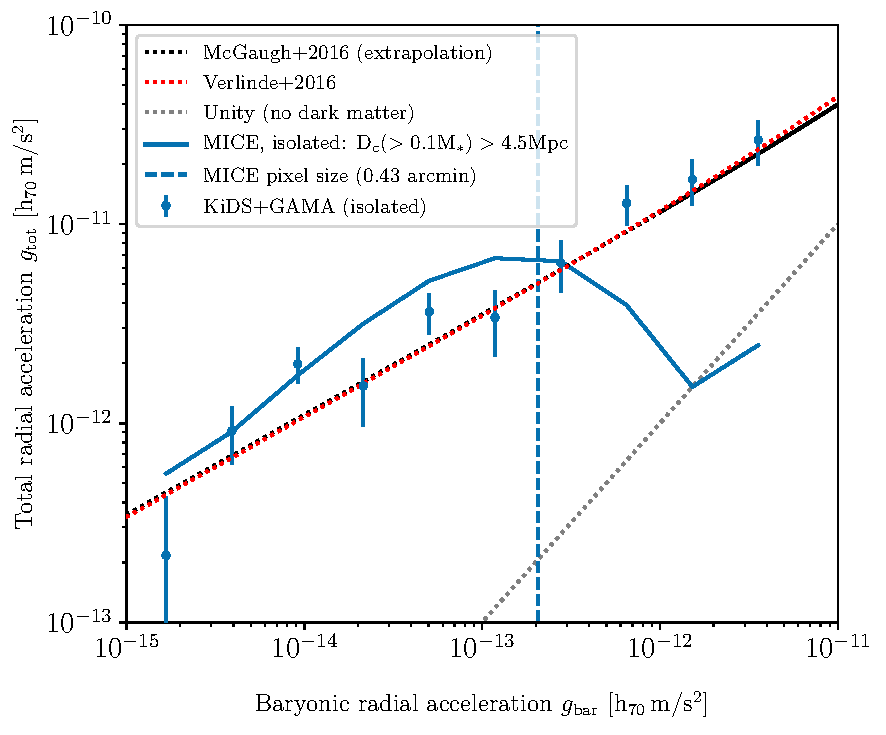
\includegraphics[width=1.0\columnwidth]{Figures/RAR_GAMA+MICE_isolated_strong.pdf}
	\caption{TBW}
	%\label{fig:}
\end{figure}

\subsection{Stellar mass bins}

\begin{figure*}
	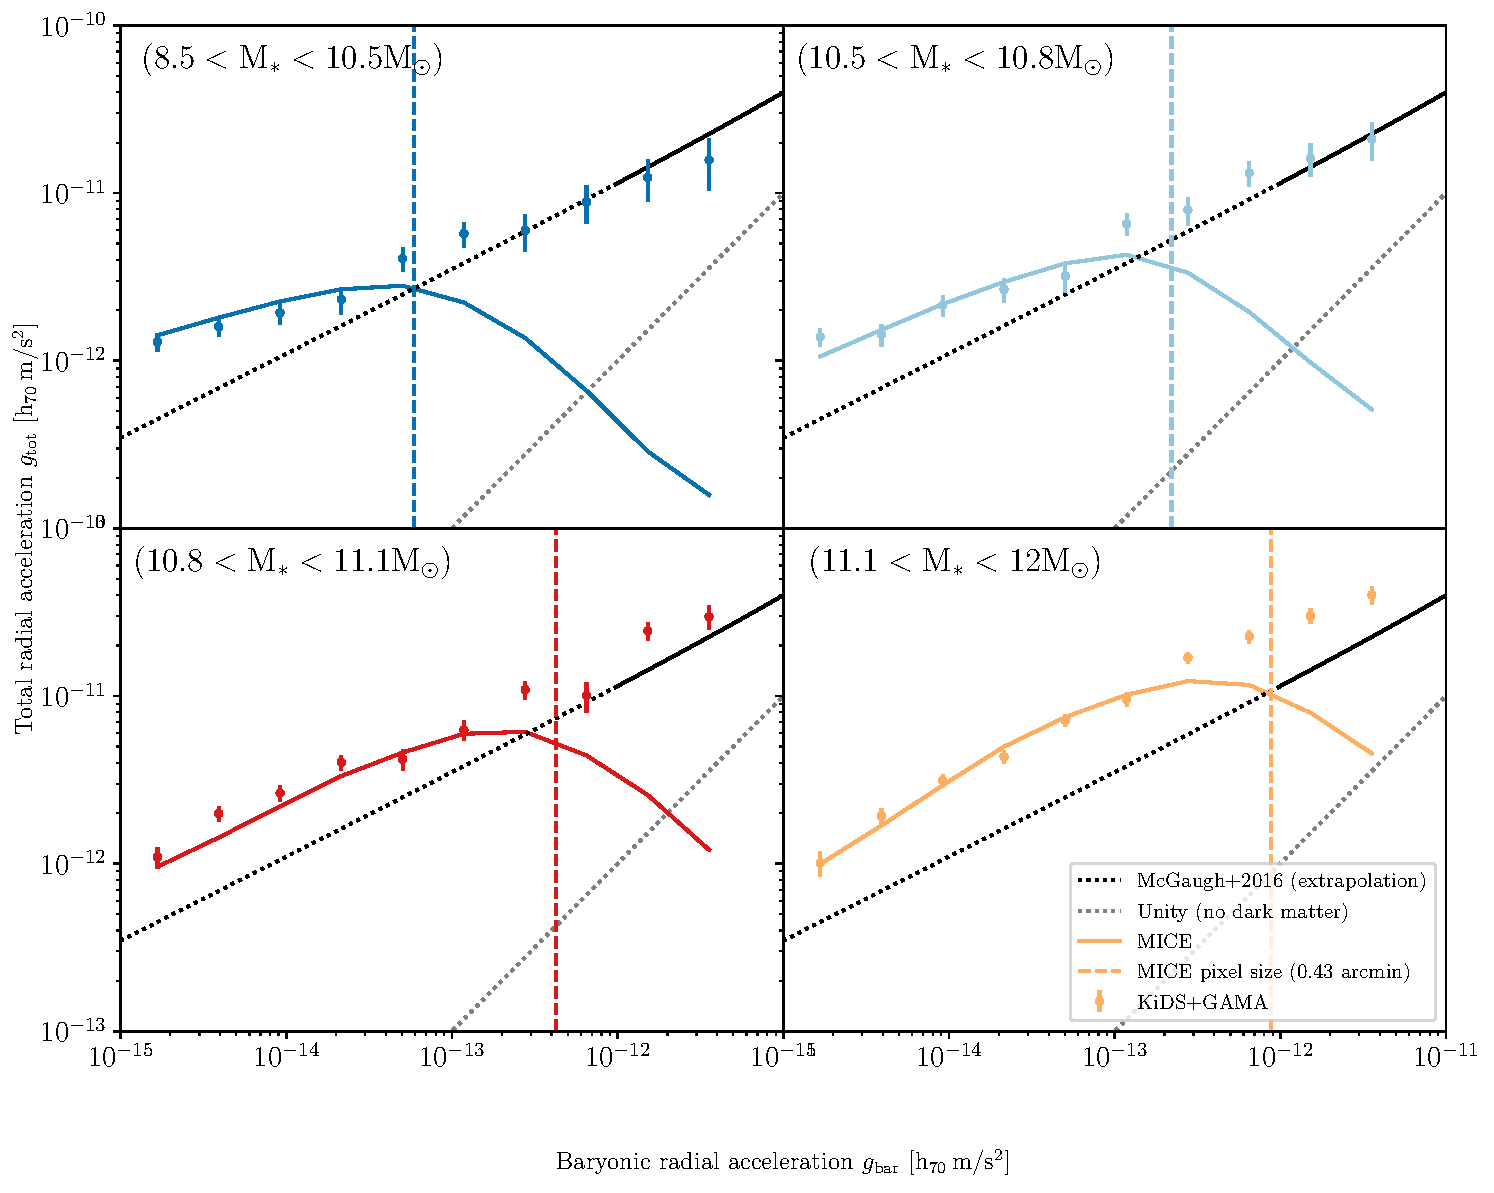
\includegraphics[width=1.0\textwidth]{Figures/RAR_GAMA+MICE_4-massbins.pdf}
	\caption{TBW}
	%\label{fig:}
\end{figure*}

\begin{figure*}
	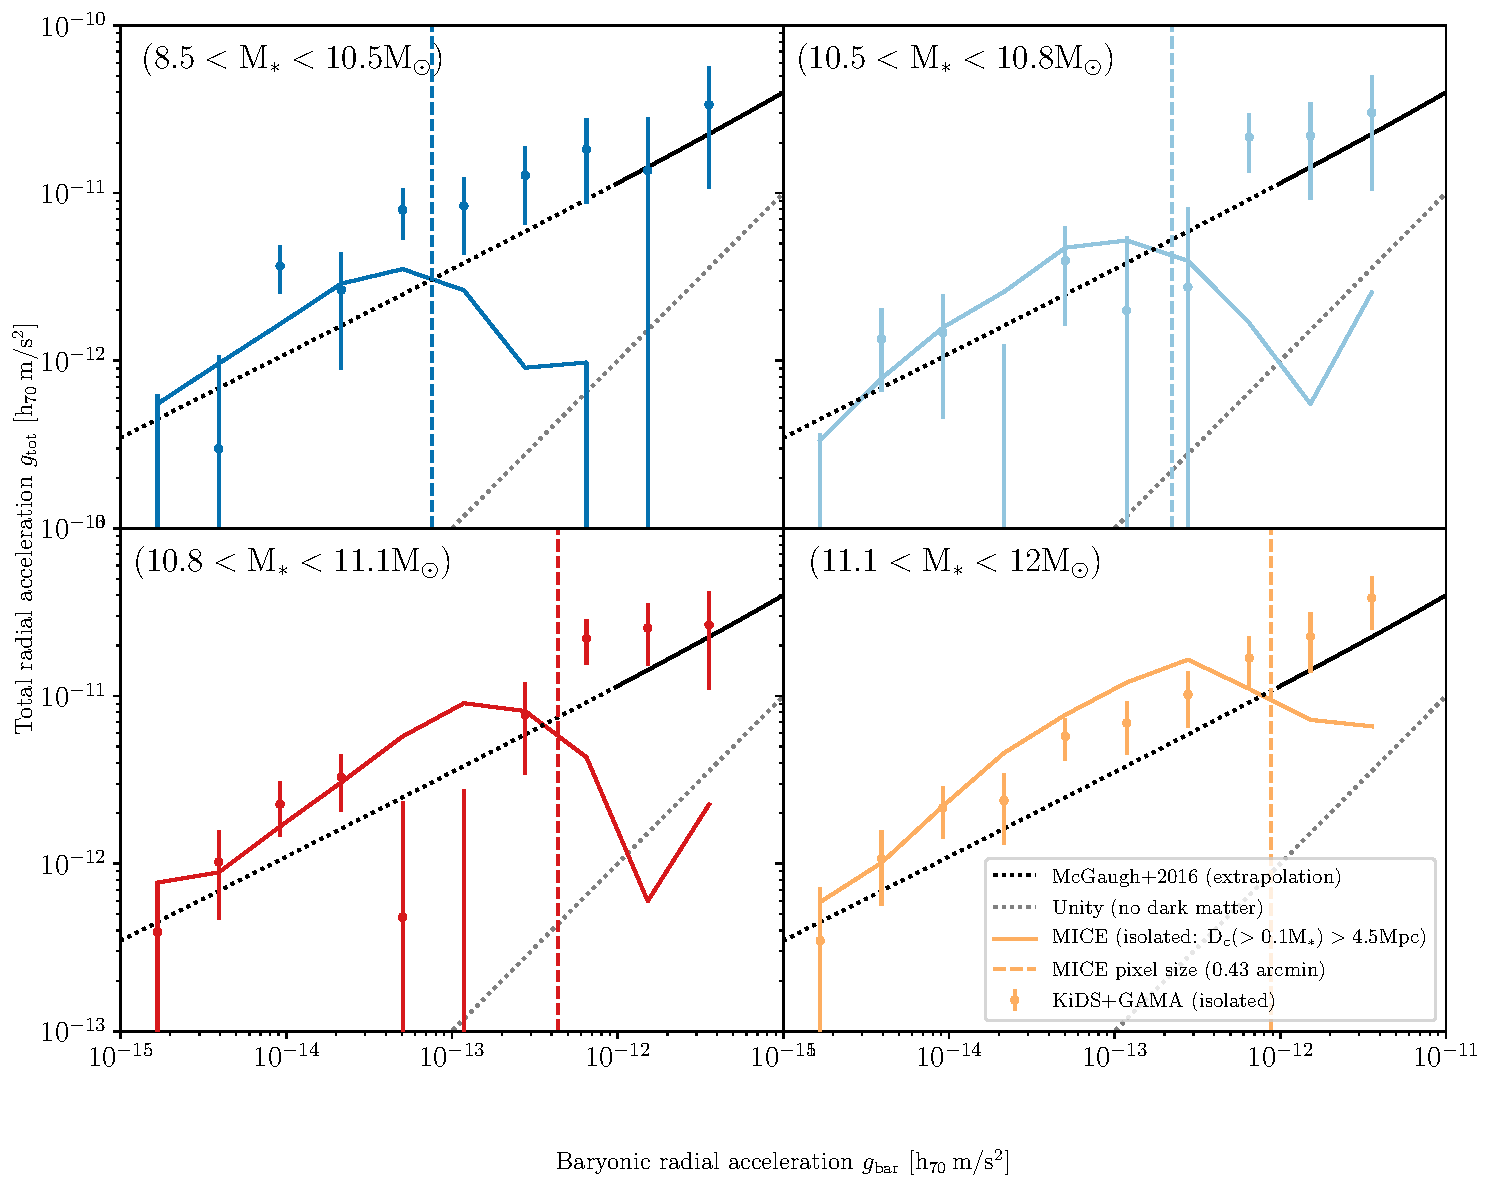
\includegraphics[width=1.0\textwidth]{Figures/RAR_GAMA+MICE_4-massbins_isolated_strong.pdf}
	\caption{TBW}
	%\label{fig:}
\end{figure*}

\begin{figure*}
	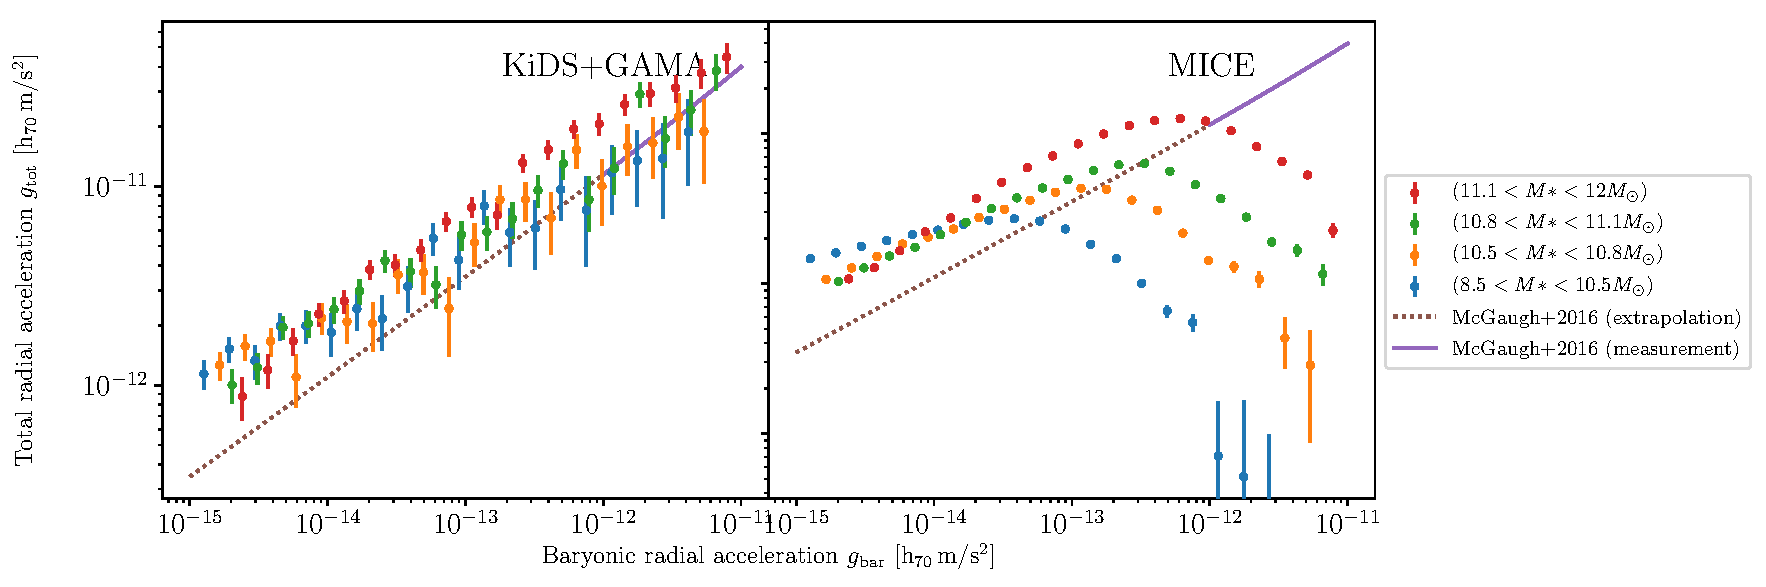
\includegraphics[width=1.0\textwidth]{Figures/RAR_KiDS+MICE_massbins-8p5_10p5_10p8_11p1_12p0_transverse.pdf}
	\caption{TBW}
	%\label{fig:}
\end{figure*}

\end{comment}


\section{Discussion and conclusion}
\label{sec:discon}
Write at the end.

\section*{Acknowledgements}
Write at the end.

\begin{comment}
V. Demchenko acknowledges the Higgs Centre Nimmo Scholarship and the Edinburgh Global Research Scholarship. J. Harnois-D{\'e}raps is supported by the European Commission under a Marie-Sk{\l}odowska-Curie European Fellowship (EU project 656869). M. Bilicki is supported by the Netherlands Organization for Scientific Research, NWO, through grant number 614.001.451. C. Heymans acknowledges support from the European Research Council under grant number 647112. H. Hoekstra acknowledges support from Vici grant 639.043.512, financed by the Netherlands Organization for Scientific Research. K. Kuijken acknowledges support by the Alexander von Humboldt Foundation. H. Hildebrandt is supported by an Emmy Noether grant (No. Hi 1495/2-1) of the Deutsche Forschungsgemeinschaft. P. Schneider is supported by the Deutsche Forschungsgemeinschaft in the framework of the TR33 `The Dark Universe'. E. van Uitert acknowledges support from an STFC Ernest Rutherford Research Grant, grant reference ST/L00285X/1.

Computations for the $N$-body simulations were performed in part on the Orcinus supercomputer at the WestGrid HPC consortium (\url{www.westgrid.ca}), in part on the GPC supercomputer at the SciNet HPC Consortium. SciNet is funded by: the Canada Foundation for Innovation under the auspices of Compute Canada; the Government of Ontario; Ontario Research Fund - Research Excellence; and the University of Toronto.

This research is based on data products from observations made with ESO Telescopes at the La Silla Paranal Observatory under programme IDs 177.A-3016, 177.A-3017 and 177.A-3018, and on data products produced by Target OmegaCEN, INAF-OACN, INAF-OAPD and the KiDS production team,  on behalf of the KiDS consortium. OmegaCEN and the KiDS production team acknowledge support by NOVA and NWO-M grants. Members of INAF-OAPD and INAF-OACN also acknowledge the support from the Department of Physics \& Astronomy of the University of Padova, and of the Department of Physics of Univ. Federico II (Naples).

GAMA is a joint European-Australasian project based around a spectroscopic campaign using the Anglo-Australian Telescope. The GAMA input catalogue is based on data taken from the Sloan Digital Sky Survey and the UKIRT Infrared Deep Sky Survey. Complementary imaging of the GAMA regions is being obtained by a number of independent survey programs including GALEX MIS, VST KiDS, VISTA VIKING, WISE, Herschel-ATLAS, GMRT and ASKAP providing UV to radio coverage. GAMA is funded by the STFC (UK), the ARC (Australia), the AAO, and the participating institutions. The GAMA website is \url{www.gama-survey.org}.

This work has made use of CosmoHub \cite[]{carretero2017}. CosmoHub has been developed by the Port d'Informaci{\'o}n Cient{\'i}fica (PIC), maintained through a collaboration of the Institut de F{\'i}sica d'Altes Energies (IFAE) and the Centro de Investigaciones Energ{\'e}ticas, Medioambientales y Tecnol{\'o}gicas (CIEMAT), and was partially funded by the ``Plan Estatal de Investigaci{\'o}n Cient{\'i}fica y T{\'e}cnica y de Innovaci{\'o}n'' program of the Spanish government.

This work has made use of {\scshape python} (\url{www.python.org}), including the packages {\scshape numpy} (\url{www.numpy.org}) and {\scshape scipy} (\url{www.scipy.org}). Plots have been produced with {\scshape matplotlib} \cite[]{hunter2007matplotlib}. The mock shear profiles from MICE are computed using {\scshape TreeCorr} (\url{https://pypi.python.org/pypi/TreeCorr}).

\emph{Author contributions:} All authors contributed to the development and writing of this paper. The authorship list is given in three groups: the lead authors (M. Brouwer, V. Demchenko, J. Harnois-D{\'e}raps), followed by two alphabetical groups. The first alphabetical group includes those who are key contributors to both the scientific analysis and the data products. The second group covers those who have either made a significant contribution to the data products, or to the scientific analysis.
end{comment}
\end{comment}
%%%%%%%%%%%%%%%%%%%%%%%%%%%%%%%%%%%%%%%%%%%%%%%%%%

%%%%%%%%%%%%%%%%%%%% REFERENCES %%%%%%%%%%%%%%%%%%

% The best way to enter references is to use BibTeX:

\bibliographystyle{mnras}
\bibliography{biblio}


%%%%%%%%%%%%%%%%%%%%%%%%%%%%%%%%%%%%%%%%%%%%%%%%%%

%%%%%%%%%%%%%%%%%%%%%%%%%%%%%%%%%%%%%%%%%%%%%%%%%%


% Don't change these lines
\bsp	% typesetting comment
\label{lastpage}
\end{document}

% End of mnras_template.tex
